\section{Parameter Study}
To gain insight into the behaviour of the RL-agent and the influence of some of the parameters, a parameter study is conducted. To reduce the effect of the random initialization of the networks, three independent agents are trained. 
\begin{figure}[h]
	\centering
	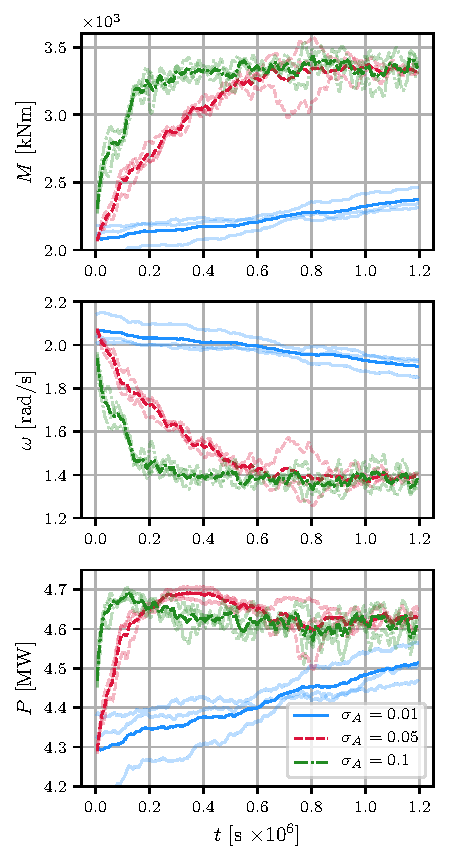
\includegraphics{variance.pdf}
	\caption{Training of RL-agent in BEM environment with different values for variance of action. Thin lines represent individual runs, thick lines are the average of all runs.}
	\label{fig:var}
\end{figure}
First the influence of the variance of the action, $\sigma_A$ is studied. The results of the training are shown in \autoref{fig:var}. The comparison of the three values shows a clear trend. A higher variance leads to a faster increase in power. Furthermore the two agents with a higher variance reach similar behaviour. They also both reach a maximum of generated power quickly, but are not able to sustain that value throughout the continued training. Comparing the different agents with the same set of parameters show that a certain stochasticity is present in training of the agents.  After around two thirds of training time, one of agents with medium variance shows a significant drop in power, while another performs significantly better than average. However, towards the end of the training, the agents with medium variance perform more similar, more stable and slightly better than the agent with a higher variance. It can therefore be assumed that the choice of variance has to be a balance between a fast increase in the beginning and unstable behaviour in the end. It can be expected that the training of the agent controlling three turbines will take significantly more timesteps and the computational cost of a single timestep is also much higher. Therefore, a faster increase is favored and a the variance is chosen to be $\sigma_A = 0.1$. \\
\begin{figure}
	\centering
	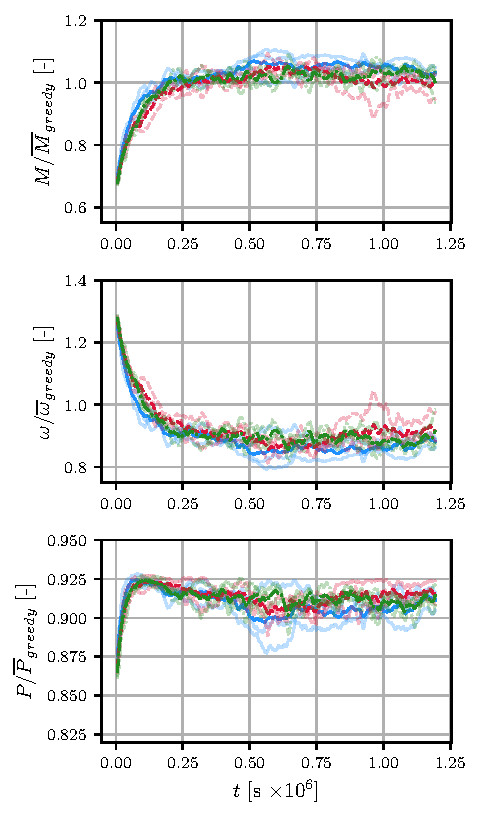
\includegraphics{policy_l2_reg.pdf}
	\caption{Training of RL-agent in BEM environment with different coefficients for policy $l_2$ regularization. Thin lines represent individual runs, thick lines are the average of all runs.}
\end{figure}